\chapter{K\"ahler-Ricci solitons on Fano threefolds} \label{chap:sol}

\chaptermark{K\"ahler-Ricci solitons on Fano threefolds}


In this chapter we prove the following theorem:
\begin{theorem}[{\cite[Theorem 1.8]{cable2018classification}}] \label{thm:sol}
The Fano threefolds \(2.30, \ 2.31, \ 3.18, \ 3.22, \ 3.23, \ 3.24, \ 4.8\) from Mori and Mukai's classification \cite{} admit a non-trivial K\"ahler-Ricci soliton.
\end{theorem}
Together with \cite[Theorems. 6.1, 6.2]{ilten2015} it follows that all known smooth Fano threefolds with an effective complexity-one torus action admit a K\"ahler-Ricci soliton. We follow the joint work of \cite{cable2018classification}. We describe here the contribution of the author to this article, namely to perform calculations to test the \(K\)-stability of threefolds and thus determine which admitted K\"ahler-Ricci solitons.

\section{Proof of Theorem \ref{thm:sol}}

Let \(X\) be a smooth complexity one Fano \(T\)-variety. Recall the definition of a K\"ahler-Ricci soliton from definition \ref{def:tKRS}. We will test for the existence of a K\"ahler-Ricci soliton on \(X\) using Theorem \ref{thm:DS}. Let \(\Phi: \Box \to \Div \PP^1\) be the divisorial polytope of \(X\) corresponding to the anticanonical polarization. 

First we use Theorem \ref{thm:BWN} to find appropriate vector fields \(\xi\). Any such \(\xi\) will satisfy the following equation: 
\begin{equation} \label{eq:producteq}
\DF_{\xi}(X \times \mathbb{A}^1, w) = 0
\end{equation}
For all \(w \in N'_\RR\). By (ref) this becomes:
\begin{equation} \label{eq:combproducteq}
(eq)
\end{equation}
By the arguments in \cite[Section~3.1]{donaldson2008kahler} there always exist a unique choice $\xi \in N_\RR$ for which this holds. We call this $\xi$ a \textit{soliton canditate}.

The integral in (\ref{eq:producteq}) may be solved symbolically, outputting an exponential polynomial \(g(\xi, e^{\xi})\) in \(\xi\). In practice however, the domain \(P\) can complicate the calculation for \(\dim X > 2\). To deal with this we developed a recursive algorithm, based on results of Barvinok (cite), which reduces the integral to evaluations at the vertices of \(P\). We explain this algorithm at the end of the chapter.

For our examples the equation \(g(\xi,e^{\xi}) = 0\) is impossible to solve analytically. To get around this we use \textit{real interval arithmetic} (RIA) estimates to find some hypercube \(D\) in which the solution \(\xi\) lies. We then use further RIA to show that \(DF>0\) on the whole of \(D\).

In the Table~\ref{solitontable} below we give the estimates found for the vector field \(\xi\) for each threefold in the list of \cite{suss2013fano}. The threefolds 3.8*, 3.21, 4.5 were shown to admit a non-trivial K\"ahler-Ricci soliton in \cite{ilten2015} Applying 
steps (\ref{item:closed-form})-(\ref{item:bounds}) from the proof of Theorem~\ref{thm:sol} provides also an approximation for the vector field \(\xi\) for these threefolds. These are included in the table, together with those threefolds shown in \cite{ilten2015} to be K\"ahler-Einstein, to show the complete picture for the Fano threefolds described in \cite{suss2013fano}. We can show that our approximations are correct to the nearest \(10^{-5}\).
%
%
%
\begin{table}[h] \centering \label{solitontable}
\captionsetup{width=.95\linewidth}
\caption{Fano threefolds and their soliton vector fields in the canonical coordinates coming with the representation of the combinatorial data in \cite{suss2013fano}.}
\begin{tabular}{l l l}
\toprule
Threefold & $\xi$ & \\ \hline
\rowstyle{\color{gray}}
Q & $(0,0)$ \\
\rowstyle{\color{gray}}
2.24* & $(0,0)$ \\
\rowstyle{\color{gray}}
2.29 & $(0,0)$ \\
2.30 & $(0,0.51489)$ \\
2.31 & $(0.28550,0.28550)$\\
\rowstyle{\color{gray}}
2.32 & $(0,0)$ \\
3.8* & $(0,-0.76905)$ \\
\rowstyle{\color{gray}}
3.10* & $(0,0)$ \\
3.18 & $(0,0.37970)$ \\
\rowstyle{\color{gray}}
3.19 & $(0,0)$ \\
\rowstyle{\color{gray}}
3.20 & $(0,0)$ \\
3.21 & $(-0.69622,-0.69622)$ \\
3.22 & $(0,0.91479)$ \\
3.23 & $(0.26618,  0.67164)$ \\
3.24 & $(0,0.43475)$ \\
\rowstyle{\color{gray}}
4.4 &  $(0,0)$ \\
4.5* &  $(-0.31043,-0.31043)$ \\
\rowstyle{\color{gray}}
4.7 &  $(0,0)$ \\
4.8 &  $(0,0.62431)$ \\
\bottomrule
\end{tabular}
\label{table:name}
\end{table}

When \(\dim  X = 2\) the process of finding suitable \(D\) via RIA is a simple application of the intermediate value theorem. For \(\dim X >2 \) we cannot immediately use the intermediate value theorem to obtain \(D\). In all but one of our examples we make use of additional symmetries to reduce to a one-dimensional problem.

Given an automorphism \(\sigma \in \GL(M)\) permuting the vertices of \(\Box\) such that \(\deg (\Phi \circ \sigma) = \deg \Phi\), by (\ref{eq:futaki-general-fibre}) we have $F_{X, \sigma^{\!*}\!(\xi)}  =  F_{X, \xi}\circ \sigma^*$. Since \(\xi \in N_\mathbb{R}\) is the unique solution to \(F_{X,\xi} = 0\), this gives \(\xi \in N_{\mathbb{R}}^{\sigma^*}\).For \(\dim X = 3\) we have \(\dim N_{\mathbb{R}}^{\sigma^*}  = 1\) and we are in a situation where intermediate value theorem may be used to find \(D\). Note that in threefold 3.23 there is no such involution, and we must take another approach, which we explain in detail in (ref).

\begin{proof}[Proof of Theorem~\ref{thm:sol}]
Note the data for this proof is collated in (ref) below. The combinatorial data for the threefolds was originally given in \cite{suss2013fano}, although the piecewise affine \(\Psi\) discussed there differs from our divisorial polytope \(\Phi\) by the divisor \(D = 2 \cdot \{ \infty \}\).

In threefolds 2.31, 3.18, 3.22, 3.24 and 4.8 $\deg \Phi$ admits a non-trivial involution which we denote $\sigma \in \GL(M)$. Choose a basis $e_1, e_2$ of $N_\RR$ with $\sigma^*(e_1)=-e_1$ and $\sigma^*(e_2)=e_2$. The soliton candidate $\xi = (\xi_1,\xi_2)$ must be contained in the line $N_\RR^{\sigma^*} = \RR e_2$. For each of these example we obtain bounds on \(\xi_2\) via the intermediate value theorem. We provide a closed form for \(h_y\) for every admissible choice of $y \in \PP^1$. By elementary estimations we provide lower bounds on \(h_y\), ensuring the positivity of $\DF_{\xi_2 e_2}(\X_{y,0,1})$.

For the case of threefold no. 3.23 there is no involution fixing $\deg \Phi$. In this case we take a more general approach to bound the value of the candidate \(\xi\). Here we make use of some elementary calculus. Note, that \(\xi\) is the unique solution to the equation \(\nabla G = 0 \), where 
\[
G(v) := \int_{\Box} \deg \bar \Phi(u) \cdot e^{\langle u, v \rangle}\, du = 
\int_{\Delta_0} e^{\langle u', (v,0) \rangle} \, du'.
\]
Now we identify a small closed rectangular region \(D \subset \RR^2 \) such that \(\nabla_n G > 0 \) holds along \(\partial D\), for \(n\) being a outer normal of the rectangle \(D\). This guarantees a solution to \(\nabla G = 0 \) in the interior of \(D\). Indeed, due to compactness, $D$ has to contain a minimum of $G$, which by our condition cannot lie on the boundary. Hence, the minimum is located in the interior and has to coincide with $\xi$, since $\nabla G$ necessarily vanishes. After bounding the value of $\xi$ we proceed with step~(\ref{item:formulae-for-DF}). 

However, for showing positivity of $\nabla_n G$ along $\partial D$ we have to use computer assistance. The approach is simple but computational intensive. First we again determine a closed form for $\nabla G_n(\xi)$ which coincides with $F_{X,\xi}(n)$ up to a positive constant. Then we subdivide the faces of the boundary in sufficiently small segments, where one of coordinates is fixed and the other varies in a small interval. Using interval arithmetic when evaluating the closed form for $\nabla_n G(\xi)$ provides the positivity result.

See also Example~\ref{exp:asymetric} for details of the computation and Appendix~\ref{App:code} for the implementation in SageMath. The complete calculations are done using SageMath and can be found as an online worksheet\footnote{CoCalc:\url{https://cocalc.com/projects/ae8e1663-e2ad-40b8-aec2-30faf4e6a54f/files/threefolds.sagews}}.
\end{proof}
\section{Two example calculations in detail}
Here we present threefolds 2.30 and 3.23 in detail:
\begin{example}[2.30 -- Blow up of quadric threefold in a point]
\label{exp:threefold}
Consider the threefold 2.30. The function \(\Phi\) is given in Figure~\ref{fig:data230}.
\begin{figure}[h]
\caption{The combinatorial data for threefold 2.30}
\label{fig:data230}
\resizebox{0.90\linewidth}{!}{
\begin{subfigure}[b]{0.30\textwidth}
\centering
  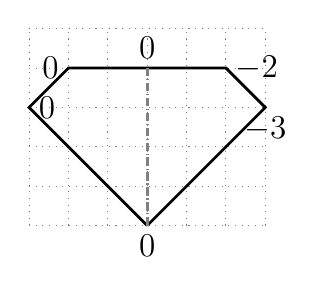
\begin{tikzpicture}[scale=0.5]
   	 \draw[dotted,step=1,gray,] (-3,-3) grid (3,2); \draw[line width = 1pt] (0,-3) --
     (-3,0) -- (-2,1)--(2,1)--
 	 (3,0)--(0,-3); \draw[densely dashdotted, gray, line width = 1.2pt] (0,-3) -- (0,1);
 	 \node at (0,-3) [below] {\large{$0$}};
 	 \node at (-3,0) [right] {\large{$0$}};
 	 \node at (-2,1) [left] {\large{$0$}};
 	 \node at (2,1) [right] {\large{$-2$}};
 	 \node at (3,0) [below] {\large{$-3$}};
 	 \node at (0,1) [above] {\large{$0$}};
	\end{tikzpicture}
	\caption*{$\Phi_0$}
\end{subfigure}
\begin{subfigure}[b]{0.30\textwidth}
	\centering
 	 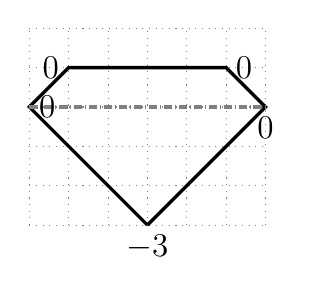
\begin{tikzpicture}[scale=0.5]
 	   \draw[dotted,step=1,gray] (-3,-3) grid (3,2); \draw[line width = 1.2pt] (0,-3) --
 	   (-3,0) -- (-2,1)--(2,1)--
 	   (3,0)--(0,-3); \draw[densely dashdotted, gray,line width = 1.2pt] (-3,0) -- (3,0);
 	 \node at (0,-3) [below] {\large{$-3$}};
 	 \node at (-3,0) [right] {\large{$0$}};
 	 \node at (-2,1) [left] {\large{$0$}};
 	 \node at (2,1) [right] {\large{$0$}};
 	 \node at (3,0) [below] {\large{$0$}};
	\end{tikzpicture}
	\caption*{$\Phi_1$}
\end{subfigure}
\begin{subfigure}[b]{0.30\textwidth}
	\centering
 	 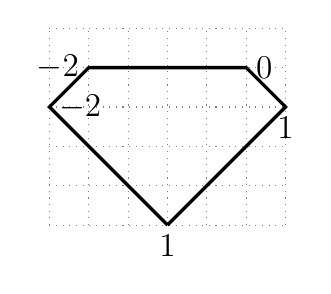
\begin{tikzpicture}[scale=0.5]
 	   \draw[dotted,step=1,gray] (-3,-3) grid (3,2); \draw[line width = 1.2pt] (0,-3) --
 	   (-3,0) -- (-2,1)--(2,1)--
 	   (3,0)--(0,-3);
 	 \node at (0,-3) [below] {\large{$1$}};
 	 \node at (-3,0) [right] {\large{$-2$}};
 	 \node at (-2,1) [left] {\large{$-2$}};
 	 \node at (2,1) [right] {\large{$0$}};
 	 \node at (3,0) [below] {\large{$1$}};
	\end{tikzpicture}
	\caption*{$\Phi_\infty$}
\end{subfigure}
\begin{subfigure}[b]{0.40\textwidth}
	\centering
 	 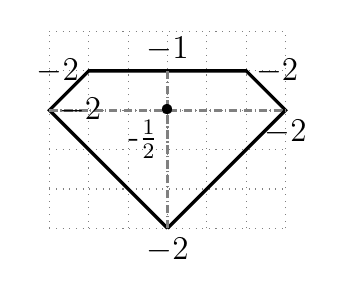
\begin{tikzpicture}[scale=0.5]
 	   \draw[dotted,step=1,gray] (-3,-3) grid (3,2); \draw[line width = 1.2pt] (0,-3) --
 	   (-3,0) -- (-2,1)--(2,1)--
 	   (3,0)--(0,-3); \draw[densely dashdotted, gray,line width = 1.2pt] (-3,0) -- (3,0); \draw[densely dashdotted, gray,line width = 1.2pt] (0,-3) -- (0,1) ;
 	 \node at (0,-3) [below] {\large{$-2$}};
 	 \node at (-3,0) [right] {\large{$-2$}};
 	 \node at (-2,1) [left] {\large{$-2$}};
 	 \node at (2,1) [right] {\large{$-2$}};
 	 \node at (3,0) [below] {\large{$-2$}};
 	 \node at (0,0) [below left] {\large{-$\frac{1}{2}$}};
 	 \node at (0,1) [above] {\large{$-1$}};
 	 \draw (0,0) node {\textbullet};
	\end{tikzpicture}
	\caption*{$\deg \Phi $}
\end{subfigure}
}
\end{figure}
We now find the unique candidate vector field \(\xi \in N_\mathbb{R}\) for a \(K\)-stable pair \((X,\xi)\). We see that $\deg \Phi$ is symmetric with respect to reflection $\sigma$ along the vertical axis. Hence, we have  \(\xi = \xi_2e_2\) for some \(\xi_2 \in \mathbb{R}\) and must find a solution $\xi_2$ to $F_{X,\xi_2e_2}=0$, which is equivalent to $F_{X,\xi_2e_2}(e_2)=0$. Indeed, we have 
\[F_{X,\xi_2e_2}(e_1) = F_{X,\sigma^*\xi_2e_2}(\sigma^*e_1)= F_{X,\xi_2e_2}(-e_1)= -F_{X,\xi_2e_2}(e_1).\]
Hence, $F_{X,\xi_2e_2}(e_1)=0$ and the claim follows by linearity.

By (\ref{eq:futaki-character}) the vanishing of $F_{X,\xi_2e_2}(e_2)$ is equivalent to that of
\[0=g(\xi_2) := \int_{\Box} u_2 \cdot \deg \bar \Phi(u) \cdot e^{u_2 \xi_2}\, du = \int_{\Delta_0} u_2 \cdot e^{u_2 \xi_2}\, du.\] Where the integral on the right hand side can be solved analytically. We obtain
\[
\frac{1}{\xi_{2}^{4}}\cdot\left({\left(2 \, \xi_{2}^{3} - 3 \, \xi_{2} - 3\right)} e^{\left(4 \, \xi_{2}\right)} + 12 \, \xi_{2} e^{\left(3 \, \xi_{2}\right)} + 3 \, \xi_{2} + 3\right) e^{\left(-3 \, \xi_{2}\right)}.
\]
Evaluating the exponential functions with a precision of 16 binary digits  and using elementary estimations it can be shown that \(g(0.514) <0\) and \(g(0.515)>0\). By the intermediate value theorem then \(0.514 < \xi_2 < 0.515\). It remains to check the positivity of the Donaldson-Futaki invariant for each degeneration. The degenerations of this threefold correspond to the polytopes:{
\begin{align*}
\Delta_0 &= \conv((-3,0,1),(-2,1,1),(2,1,-1),(3,0,-2),(0,-3,1),(0,1,1)); \\
\Delta_1 &= \conv((-3,0,1),(-2,1,1),(0,1,0),(2,1,1),(3,0,1),(0,-3,-2)); \\ 
\Delta_\infty &= \conv((-3,0,-1),(-2,1,-1),(2,1,1),(3,0,2),(0,-3,2),(0,0,-1),(0,1,-1)); \\
\Delta_y &= \conv((0, 0, -1/2), (3, 0, 1), (2, 1, 1), (0, 1, 0), (-2, 1, 1), (-3, 0, 1), (0, -3, 1)) \\ 
& \ \ \ ( \text{for } y 
\not \in \{0,1,\infty\} ).
\end{align*}}
In each case we have induced \(\CC^*\)-action given by \((0,0,1) \in N \times \ZZ \). Denote
\[
h_y(\xi_2) := (\vol \Delta_y) \cdot \DF_{(0,\xi_2)}(\X_{y,0,1}).
\]
Clearly positivity of \(h_y\) implies the positivity of \(\DF_\xi(\X_{y,0,1})\). 
Once more solving the integrals appearing in (\ref{eq:futaki-character}) analytically with $y \not \in \{0,1,\infty\}$  we obtain:
\begin{align*}
h_0(\xi_2) &= \frac{1}{3\xi_2^{4}}\cdot
{\left({\left(2   \xi_2^{3} - 3   \xi_2 - 3\right)} e^{4   \xi_2} + 3   {\left(3   \xi_2^{2} + 2\right)} e^{3   \xi_2} - 3   \xi_2 - 3\right)} e^{-3   \xi_2}
\\
h_1(\xi_2) &= \frac{1}{6   \xi_2^{4}}\cdot
{\left({\left(8   \xi_2^{3} + 6   \xi_2^{2} - 3\right)} e^{4   \xi_2} - 12   {\left(3   \xi_2^{2} - 3   \xi_2 + 1\right)} e^{3   \xi_2} + 12   \xi_2 + 15\right)} e^{-3   \xi_2} \\
h_\infty(\xi_2) &= -\frac{1}{6   \xi_2^{4}}\cdot
{\left(2   {\left(2   \xi_2^{3} - 3   \xi_2 - 3\right)} e^{4   \xi_2} - 3   {\left(3   \xi_2^{2} - 12   \xi_2 + 2\right)} e^{3   \xi_2} + 12   \xi_2 + 12\right)} e^{-3   \xi_2} \\
h_y(\xi_2) &= \frac{1}{6   \xi_2^{4}}\cdot{\left({\left(8   \xi_2^{3} + 6   \xi_2^{2} - 3\right)} e^{4   \xi_2 } - 3   {\left(3   \xi_2^{2} - 2\right)} e^{3   \xi_2} - 6   y - 3\right)} e^{-3   \xi_2} 
\end{align*}

Using the same precision as above for the  evaluations of the exponential functions at the lower and upper bounds for \(\xi_2\) gives estimates:
\begin{align*}
1.087 &< h_0(\xi_2) < 1.458 \\
2.178 &< h_1(\xi_2) < 2.470 \\
0.446 &< h_\infty(\xi_2) < 0.827 \\
4.151 &< h_y(\xi_2) < 4.309 \ \ \ \ \ \ \   \left( \text{for } y \not \in \{0,1,\infty\} \right)
\end{align*}
We can therefore conclude that the threefold 2.30 is \(K\)-stable, and must admit a non-trivial K\"ahler-Ricci soliton.
\end{example}

\begin{example}[3.23 -- Blowup of the quadric in a point and a line passing through]
\label{exp:asymetric}
We follow the calculations outlined in the above proof of Theorem~\ref{thm:sol}. As before we first have to find a closed form for $F_{X,\xi}(n)$ or $\nabla_n G(\xi)$, respectively. Then numerically we can find an approximation to \(\xi\) as the point:
\[
(x_0,x_1) = (0.26617786,  0.67164063).
\]
Setting \(\epsilon = 10^{-5}\), consider the square containing our approximation, given by:
\[
D = [x_0 - \epsilon,x_0+\epsilon] \times [x_1 - \epsilon, x_1 + \epsilon]
\]
Subdividing each edge of the boundary \(\partial D\) into line segments of length \(\epsilon/1500\), we use interval arithmetic to verify that the gradient of \(h\) is positive in the outer normal direction for each of these segments, in fact \(\nabla_n G > 5.536 \cdot 10^{-6}\) along \(\partial D\). Once again it remains to check the positivity of the Donaldson-Futaki invariant for each degeneration. The degenerations of this threefold correspond to the polytopes:
{
\
 \begin{align*}
\Delta_0 &= \conv((-3,0,1),(-2,1,1),(0,1,0),(0,1,1),(1,1,0),(2,0,-1),(2,-1,-1),\\
         &\qquad  (0,-3,1),(1,0,-1)); \\
\Delta_1 &= \conv((-3,0,1),(-2,1,1),(1,1,1),(2,0,1),(2,-1,0),(0,-3,-2),(0,1,0)); \\ 
\Delta_\infty &= \conv((-3,0,-1),(-2,1,-1),(0,1,0),(1,1,0),(2,0,1),(2,-1,2),(0,-3,2),\\
&\qquad (0,1,-1),(0,0,-1)) \\
\Delta_y &= \conv((0, 0, -1/2), (0, 1, 0), (1, 0, 0), (1, 1, 1), (2, 0, 1), (2, -1, 1), \\ & \qquad (-2, 1, 1), (-3, 0, 1), (0, -3, 1)) \ \ \  ( \text{for } y 
\not \in \{0,1,\infty\} ).
\end{align*}}
Interval arithmetic gives the following lower bounds on the Donaldson-Futaki invariants:
\begin{align*}
h_0(\xi_2) &> 1.2766 \\
h_1(\xi_2) &> 1.8401 \\
h_\infty(\xi_2) &> 0.1004 \\
h_y(\xi_2) &> 3.4443 \ \ \  ( \text{for } y 
\not \in \{0,1,\infty\} )
\end{align*}
We can therefore conclude that the threefold 3.23 is \(K\)-stable, and must admit a non-trivial K\"ahler-Ricci soliton. See also Appendix~\ref{App:code} for the SageMath code of the calculations.
\end{example}

\section{Barvinok Integration}
The integral (ref) may be solved symbolically, outputting an exponential polynomial in \(\xi\). In practice however, the domain \(P\) can complicate the calculation for \(\dim X > 2\). To deal with this we developed a recursive algorithm, based on results of Barvinok (cite), which reduces the integral to evaluations at the vertices of \(P\). Here we explain how this algorithm works.
\[
\int_{P} l_1(x) e^{l_2(x)}
\]
for some linear functions \(l_1,l_2\). If we were working with surfaces, as is done earlier in \cite{cable2018classification}, then \(P\) is just an interval and the integral can be computed easily by hand. In theory one could divide and parameterize the domain for higher dimensions, but this quickly makes the process of integration a very tedious task for even mildly complicated domains \(P\).

In \cite{barvinok} Stoke's theorem is applied to a polytope domain. We may use this to iteratively reduce the dimension of our problem by rewriting the integral as an integral over the facets of \(P\).

\begin{example}
example of Barvinok algorithm
\end{example}	